\thispagestyle{empty}

\vspace*{0.25in}
{\sffamily\bfseries\fontsize{48}{48}\selectfont\color{TitoInk}TITO\par}
\vspace{2pt}
{\sffamily\bfseries\fontsize{25}{28}\selectfont\color{TitoRule}
  Playbook\par}
\vspace{7pt}
{\sffamily\bfseries\fontsize{18}{21}\selectfont\color{TitoRed}
  A Scripted Example of Play\par}
{\sffamily\large Game-Turns 1--5\par}

\vspace{10pt}
{\color{TitoInk}\hrule height 1.2pt}
\vspace{9pt}

\begin{center}
  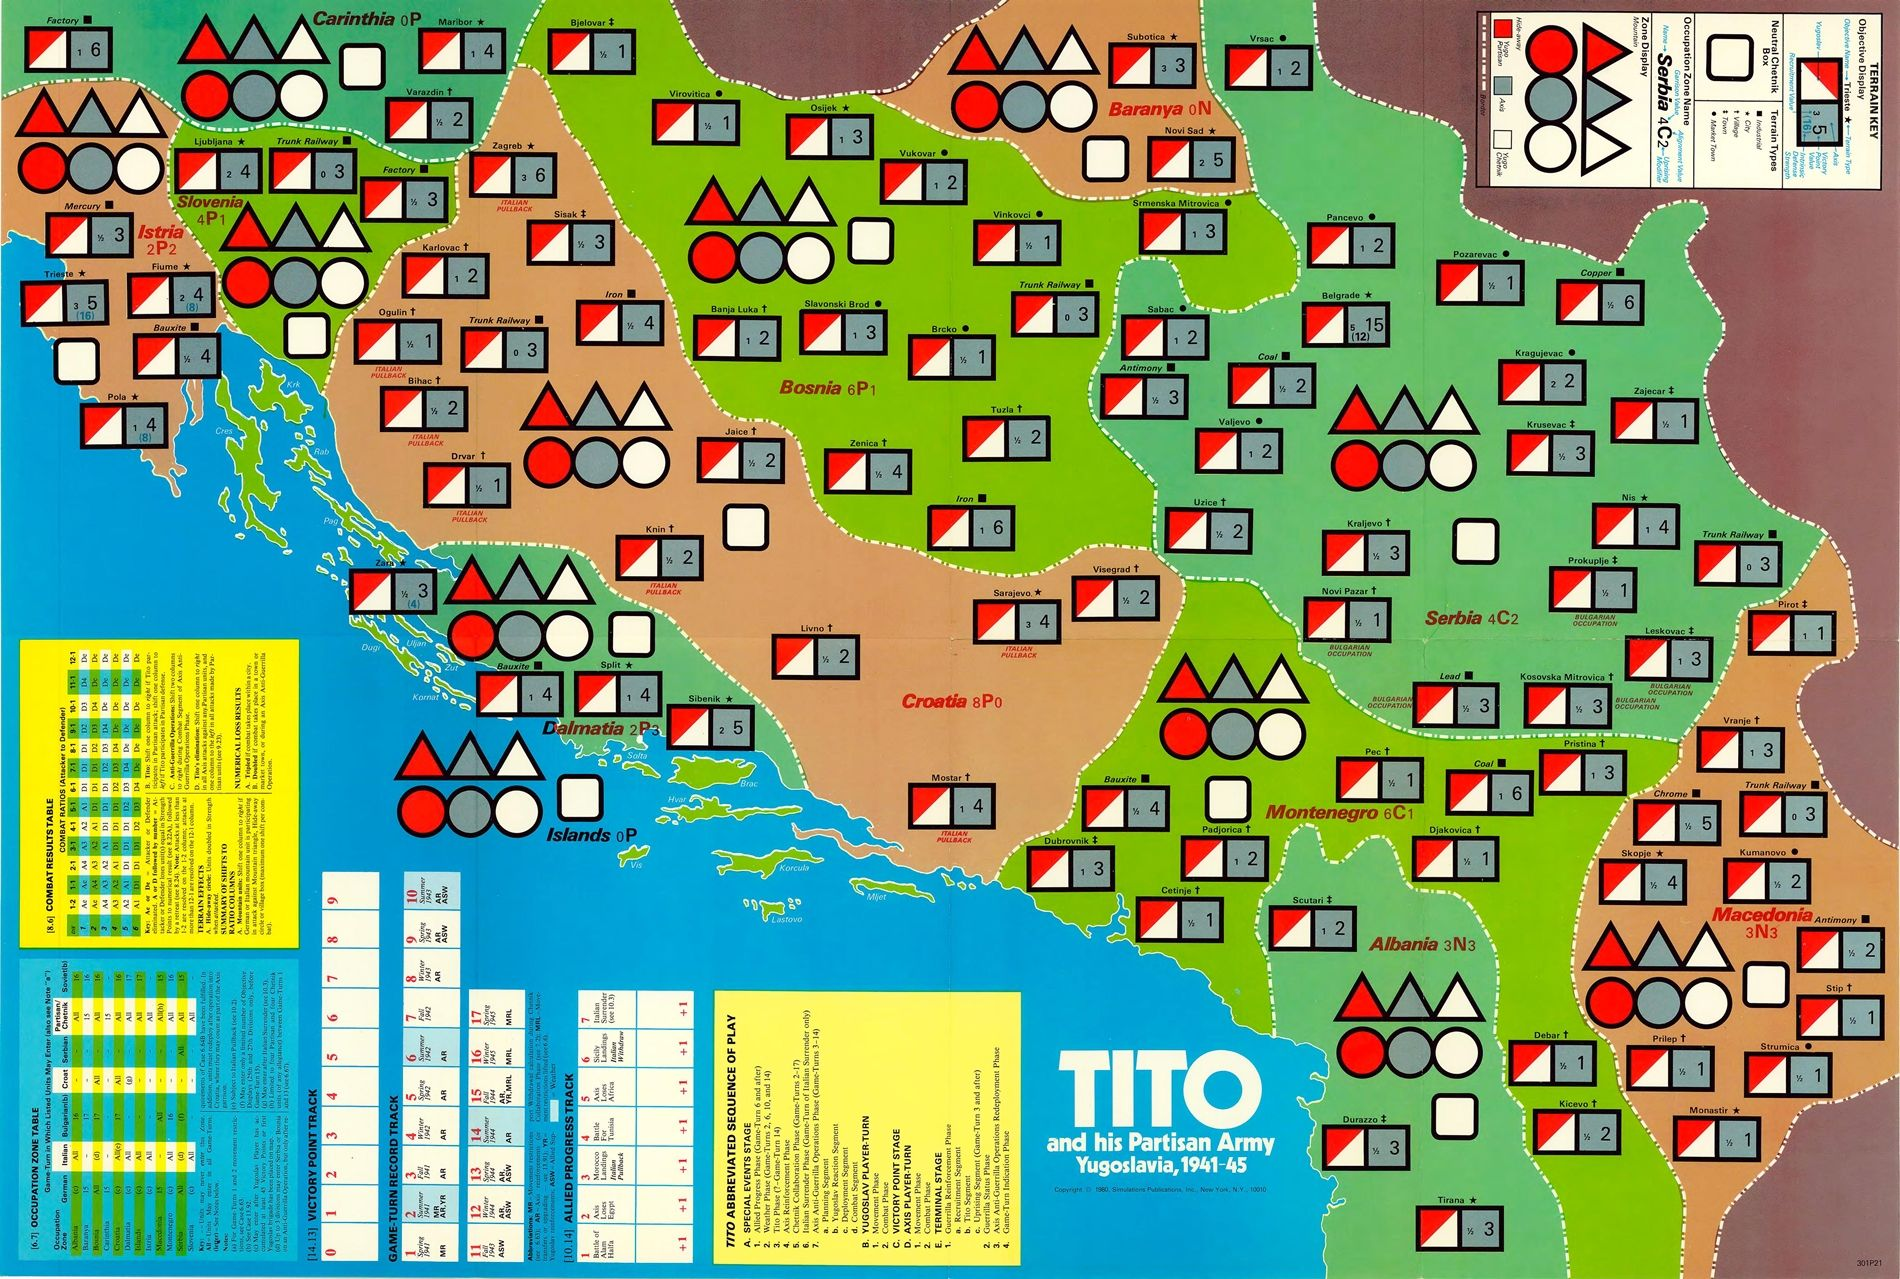
\includegraphics[width=0.96\linewidth,trim=0 105 0 0,clip]
    {../../Misc/Images/Tito/tito_map.jpg}
\end{center}

\vfill
\begin{minipage}[t]{0.57\textwidth}
  \small
  This playbook teaches the opening of \emph{Tito} by walking through a
  deliberately scripted game. The decisions are legal and plausible, but they
  are chosen to demonstrate systems rather than provide perfect strategy.
  Follow the stated setup and use the printed die rolls to reproduce the
  example at the table.
\end{minipage}
\hfill
\begin{minipage}[t]{0.37\textwidth}
  \raggedleft
  {\sffamily\bfseries Presentation by Daniel J. Berger\par}
  {\sffamily Version 0.1\par}
  {\sffamily \today\par}
\end{minipage}

\clearpage

\section{How to Use This Playbook}

\begin{multicols}{2}
\small
The example follows the complete Sequence of Play, but compresses phases in
which no choice or game-state change occurs. Every prescribed die roll is
shown in a red box. Rules citations point to the restored rulebook.

The map illustrations are snapshots, not stack inventories. Numbered callouts
match the accompanying prose; exact stacks are stated in the text and in each
turn ledger. Counters are not drawn to scale.

\begin{lessonbox}
\begin{itemize}[leftmargin=1.2em,itemsep=2pt]
  \item Game-Turn 1: movement, objectives, combat, retreat, and recruitment.
  \item Game-Turn 2: drought, Chetnik collaboration, and Tito.
  \item Game-Turn 3: Anti-Guerrilla Operations and uprisings.
  \item Game-Turn 4: winter, brigade formation, and expanded Axis movement.
  \item Game-Turn 5: locating Tito and an elimination attempt.
\end{itemize}
\end{lessonbox}

\columnbreak

\subsection{Contents}

\begin{tabularx}{\linewidth}{@{}Xr@{}}
  Preparing the Game & 3 \\
  Game-Turn 1: Testing the Occupation & 4 \\
  Game-Turn 2: Tito Enters the War & 5 \\
  Game-Turn 3: The War Spreads & 6 \\
  Game-Turn 4: Winter and Escalation & 8 \\
  Game-Turn 5: The Hunt for Tito & 9 \\
  After Five Turns & 10 \\
\end{tabularx}

\subsection{Conventions}

\begin{tabularx}{\linewidth}{@{}>{\bfseries}l X@{}}
  P & Partisan \\
  C & Chetnik \\
  Y/A/N & pro-Yugoslav, pro-Axis, neutral \\
  SP & Combat Strength Points \\
  AGO & Anti-Guerrilla Operation \\
  GT & Game-Turn \\
\end{tabularx}

\begin{commentarybox}
This tutorial uses the original restored rules. It does not employ the
unverified online addenda.
\end{commentarybox}
\end{multicols}

\vfill
\begin{center}
  \counterpic[0.62in]{german-infantry-front}\hspace{0.13in}
  \counterpic[0.62in]{chetnik-group}\hspace{0.13in}
  \counterpic[0.62in]{tito-unidentified}\hspace{0.13in}
  \counterpic[0.62in]{partisan-group}\hspace{0.13in}
  \counterpic[0.62in]{partisan-brigade}
\end{center}
